\section{Berechnungsprozess}
Die Berechnung eines optimalen Stosses wird aufgrund der vielen Möglichkeiten sehr zeitintensiv, weswegen
die expandierten Teilschritte parallel gerechnet werden.

\begin{figure}[h!]
    \begin{center}
        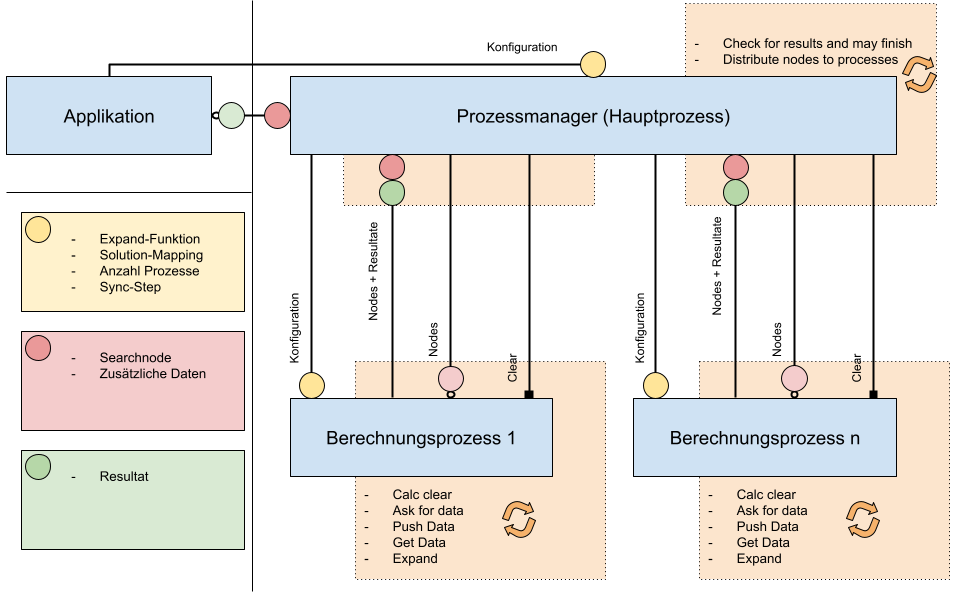
\includegraphics[width=0.8\linewidth]{../common/03_billiard_ai/resources/14_berechnungsprozess.png}
    \end{center}
    \caption{Berechnungsprozess}
    \label{fig:berechnungsprozess}
\end{figure}

Abbildung \ref{fig:berechnungsprozess} erläutert die Durchführung dieser Expansionsschritte.
Die Applikation auf der linken Seite liefert die konkreten Aufgaben, welche von einem Pool an Berechnungsprozessen
bearbeitet werden sollen. Sie beinhaltet die Logik, um eine solche Aufgabe zu lösen, da die Berechnungsprozesse
selbst nicht über dieses Wissen verfügen.
Der Pool von Berechnungsprozessen wird vom Prozessmanager verwaltet und dieser ist die zentrale Ansprechperson der Applikation.

Datenaustausche sind über gefärbte Kreise repräsentiert. Handelt es sich um einen asynchronen
Datenaustausch, dann ist der entsprechende Kreis heller eingefärbt und die Verbindungslinie ist durch einen nicht
ausgefüllten Punkt gekennzeichnet. Es werden die Farben Rot den zu bearbeitenden Daten,
Gelb den Konfigurationsdaten und Grün den Resultaten zugeordnet. Signale sind durch ein ausgefülltes Quadrat an der
Verbindungslinie gekennzeichnet. Das Signal oder die Daten sind jeweils beim Empfänger angegeben. Repetitive Aufgaben
sind durch ein hinterlegtes oranges Rechteck markiert.

Bei der Erstellung des Prozessmanagers werden alle Konfigurationen mitgeliefert. Der Prozessmanager erzeugt während seiner
Instanziierung die Prozesse, welche ebenfalls direkt konfiguriert werden. Die Prozesse laufen nun im Hintergrund und
warten auf Daten.

Erhält die Applikation eine Suchanfrage, ruft sie in einem ersten Schritt den Prozessmanager auf.
Dieser nimmt noch zu berechnende Daten entgegen. Im Fall von Billard sind dies die Root-Nodes des Suchbaums.
Jeder Root-Node repräsentiert ein Loch. Der Prozessmanager gibt in dem Fall eine Datenstruktur zurück, welche es erlaubt,
in Zukunft auf die Anfrage zu antworten. In dieser Antwort werden die Resultate geliefert.
Der Hauptprozess prüft regelmässig, ob die Bearbeitung der gestellten Aufgaben beendet werden soll.
Dies ist der Fall, wenn entweder genügend Lösungen gefunden wurden, die maximal zur Verfügung stehende Zeit abgelaufen ist
oder keine noch zu expandierenden Nodes mehr vorhanden sind.
Sollte die Berechnung nicht abgebrochen werden, dann werden die offenen Anfragen der Berechnungsprozesse beantwortet.
Der Prozessmanager verteilt alle ihm gemeldeten noch zu bearbeitenden Daten an die einzelnen Berechnungsprozesse.

In Abbildung \ref{fig:berechnungsprozess_verteilung} wird das Ziel verdeutlicht, welches der Prozessmanager bei einer
Verteilung dieser Daten verfolgt. So sollen die jeweils $n$ besten Kandidaten, wobei $n$ für die Anzahl der Berechnungsprozesse
steht, auf die verschiedenen Berechnungsprozesse verteilt werden. Danach erhalten die Berechnungsprozesse die nächstbesten
$n$-Kandidaten. Dadurch wird sichergestellt, dass immer an den vielversprechendsten Arbeitspaketen weitergemacht wird.

\begin{figure}[h!]
    \begin{center}
        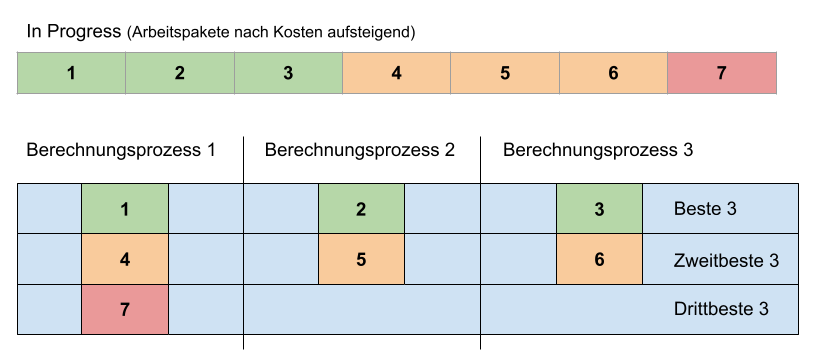
\includegraphics[width=0.8\linewidth]{../common/03_billiard_ai/resources/20_berechnungsprozess_verteilung.png}
    \end{center}
    \caption{Berechnungsprozessverteilung}
    \label{fig:berechnungsprozess_verteilung}
\end{figure}

Der Algorithmus \ref{alg:distribute_manager} zeigt, wie die offenen Arbeitspakete auf die Berechnungsprozesse verteilt
werden, damit das Ziel in Abbildung \ref{fig:berechnungsprozess_verteilung} erreicht werden kann. So werden
zuerst alle Antworten auf die offenen Anfragen erstellt. Dies geschieht in einer \glqq While-Loop\grqq, welche so lange
läuft, wie es noch offene Arbeitspakete hat. In jedem Schritt der Schleife wird ein Arbeitspaket einer Antwort für eine
Anfrage hinzugefügt. Am Ende der Schleife wird eine Index-Variable hochgezählt. Sollte diese die Anzahl der offenen Anfragen
erreichen, beginnt sie wieder bei 0. Dies ist z.B. in Abbildung \ref{fig:berechnungsprozess_verteilung} beim Wechsel von
Arbeitspakte $3$ zu $4$ ersichtlich. Sobald keine offenen Arbeitspakete mehr existieren, werden sämtliche Anfragen
beantwortet, zu welchen Antworten erstellt werden konnten. Wenn z.B. mehr Anfragen als Arbeitspakete existieren, bleiben
diese erhalten und werden im nächsten Synchronisationszyklus beantwortet\footnote{Man stelle sich bei der Abbildung
\ref{fig:berechnungsprozess_verteilung} nur zwei offene Arbeitspakete vor. Demnach würde Paket $1$ auf den Berechnungsprozess
    $1$ und Paket $2$ auf den Berechnungsprozess $2$ verteilt werden. Die Anfrage des Berechnungsprozesses $3$ bliebe offen.}.
\begin{algorithm}[H]
    \DontPrintSemicolon
    \SetKwFunction{distribute}{distribute}
    \SetKwProg{Fn}{Function}{}{}
    \Fn{\distribute{requests: List[future], inProgress: Queue[Node]} $\longrightarrow$ List[future]}{
        answers: List[List[Node]] $\longleftarrow$ list()\\
        forRequest $\longleftarrow$ 0\\
        \While{! inProgress.empty()}{
            \If{answers[forRequest] is null}{
                answers[forRequest] = list()
            }

            node $\longleftarrow$ pop(inProgress)\\
            answers[forRequest] $\longleftarrow$ append(node, answers[forRequest])\\
            forRequest $\longleftarrow$ (forRequest + 1) \% size(requests)
        }

        \While{! answers.empty()}{
            request $\longleftarrow$ pop(requests)\\
            fulfill(request, pop(answers))
        }

        \KwRet requests
    }
    \caption{Algorithmus zur Durchführung eines Expansionsschritts im Berechnungsprozess}
    \label{alg:distribute_manager}
\end{algorithm}

In einem Zyklus eines Berechnungsprozesses wird zuerst geprüft, ob eine Berechnung abgebrochen werden soll. Dies ist der
Fall, wenn der Prozessmanager ein \glqq Clear-Signal\grqq{} gesendet hat. Dieses Signal tritt auf, wenn eine neue
Berechnung gestartet oder wenn eine aktuell Laufende erfolgreich beendet oder abgebrochen wird.

Der Berechnungsprozess stellt in einem nächsten Schritt eine Datenanfragen an den Prozessmanager, sollte keine offene oder
noch nicht bearbeitete Anfrage existieren. Danach erfolgt die Prüfung, ob die Zeit zwischen einem Synchronisationsschritt
abgelaufen ist. In dem Fall liefert der Berechnungsprozess seine besten weiterzuführenden Berechnungen wie auch Resultate
dem Prozessmanager. Er wird demnach für eine Weile an weniger erfolgversprechenden Resultaten weiterarbeiten. In einem
weiteren Schritt wird geprüft, ob eine Datenanfrage bereits beantwortet wurde. Ist dies der Fall, so werden die
Daten den zu bearbeitenden Daten des Berechnungsprozesses hinzugefügt. Zuletzt erfolgt der Expansionsschritt, wobei der
erfolgversprechendste Kandidat expandiert wird.
Der Algorithmus \ref{alg:expand_berechnung} zeigt, wie dies in etwa funktionieren kann.
Als Eingabe dient eine priorisierte Queue von offenen Arbeitspaketen sowie die Implementation der \glqq Expand-Funktion\grqq.
Wenn es offene Arbeitspakete gibt, dann wird das Beste genommen und über die Implementation der
\glqq Expand-Funktion\grqq{} expandiert. Das Resultat dieses Schrittes wird danach entweder den Lösungen oder den
offenen Arbeitspaketen hinzugefügt. Am Schluss werden die offenen Arbeitspakete wie auch die Lösungen zurückgegeben.

\begin{algorithm}[H]
    \DontPrintSemicolon
    \SetKwFunction{expand}{expand}
    \SetKwProg{Fn}{Function}{}{}
    \Fn{\expand{inProgress: Queue[Node], expandImpl: functional} $\longrightarrow$ Queue[Node], Queue[Node]}{
        solutions $\longleftarrow$ priority\_queue()\\
        \If{!inProgress.empty()}{

            node $\longleftarrow$ pop(inProgress)\\
            expandedNodes $\longleftarrow$ expandImpl(node)\\

            \For{expandedNode in expandedNodes}{
                \If{expandedNode.isSolution()}{
                    solutions $\longleftarrow$ append(expandedNode, solutions)
                }
                \Else{
                    inProgress $\longleftarrow$ append(expandedNode, inProgress)
                }
            }
        }

        \KwRet inProgress, solutions
    }
    \caption{Algorithmus zur Durchführung eines Expansionsschritts im Berechnungsprozess}
    \label{alg:expand_berechnung}
\end{algorithm}

Die Synchronisation zwischen den Prozessen wird in Abbildung \ref{fig:berechnungsprozess_synchronisation} erläutert.
Sie findet nach einer konfigurierten Zeit $k$ statt. Diese wird in Millisekunden $[ms]$
angegeben. Da die Synchronisation ein exklusives Verwenden einer geteilten Ressource erfordert, um die erledigte Arbeit
dem Prozessmanager mitzuteilen, erhalten alle laufenden Prozesse (dies umfasst den Hauptprozess des Prozessmanagers wie auch
alle Berechnungsprozesse) ein Zeitfenster zugeteilt, welches nach $k$ Millisekunden startet. Danach kann jeder Prozess nach
$k + i \cdot n$, wobei $i$ für die Prozess-ID beginnend bei $0$ und $n$ für das Zeitfenster einer Synchronisation steht,
mit der Synchronisation beginnen. Es wird so verhindert, dass zu viele Prozesse auf die Ressource des Prozessmanagers
warten müssen und untätig bleiben. Ein weiterer Vorteil dabei ist die Tatsache, dass in der Zeit der Synchronisation
einige Prozesse Zeit erhalten, um eher schlechter bewertete Kandidaten weiterzuverfolgen. Dadurch ist es möglich,
dass ein sehr gutes Ergebnis gefunden werden kann, obwohl dessen Kandidat anfänglich als schlecht beurteilt wurde.

\begin{figure}[h!]
    \begin{center}
        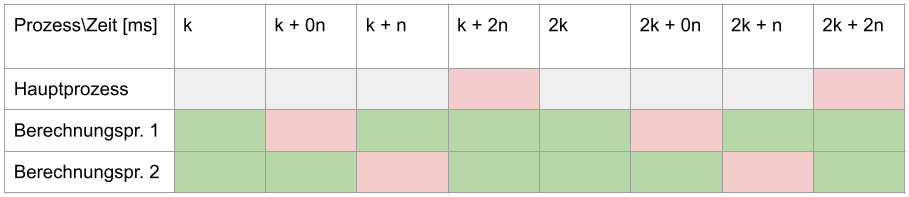
\includegraphics[width=0.8\linewidth]{../common/03_billiard_ai/resources/15_berechnungsprozess_synchronisation.png}
    \end{center}
    \caption{Berechnungsprozesssynchronisation}
    \label{fig:berechnungsprozess_synchronisation}
\end{figure}

Die Abbildung \ref{fig:berechnungsprozess_synchronisation} zeigt den Hauptprozess wie auch zwei Berechnungsprozesse, welche
eine Synchronisation in einem Intervall von $k$ Millisekunden durchführen. Grüne Spalten stehen hierbei für die Zeit, welche für die Berechnung
einer Lösung verwendet wird, also als produktiv bezeichnet werden kann. Rote Spalten hingegen signalisieren den unproduktiven
Overhead, der bei der Synchronisation entsteht. Der Prozessmanager macht nebst seinem Synchronisationsfenster nichts,
weswegen seine Spalten grau markiert sind. Eine mögliche Verbesserung wäre die Auslastung des Prozessmanagers mit zusätzlicher
Berechnungsarbeit, wie sie die Berechnungsprozesse durchführen.
